In Section~\ref{sec:metric} we show multiple ways of endowing the mapping space with a distance metric.
A common method for defining a metric in a \ac{NoC}-based system is to count the number of hops between two processors~\cite{singh2010communication,schwarzer2017symmetry}.
Indeed, this is the same as the $L_1$ (Manhattan) distance on the topology graph of the architecture.
A natural idea that arises from this is to search for \emph{compact} mappings\index{compact mappings}, i.e. mappings that take a (geometrically) small area in the chip.


\begin{figure*}[th]
	\centering
	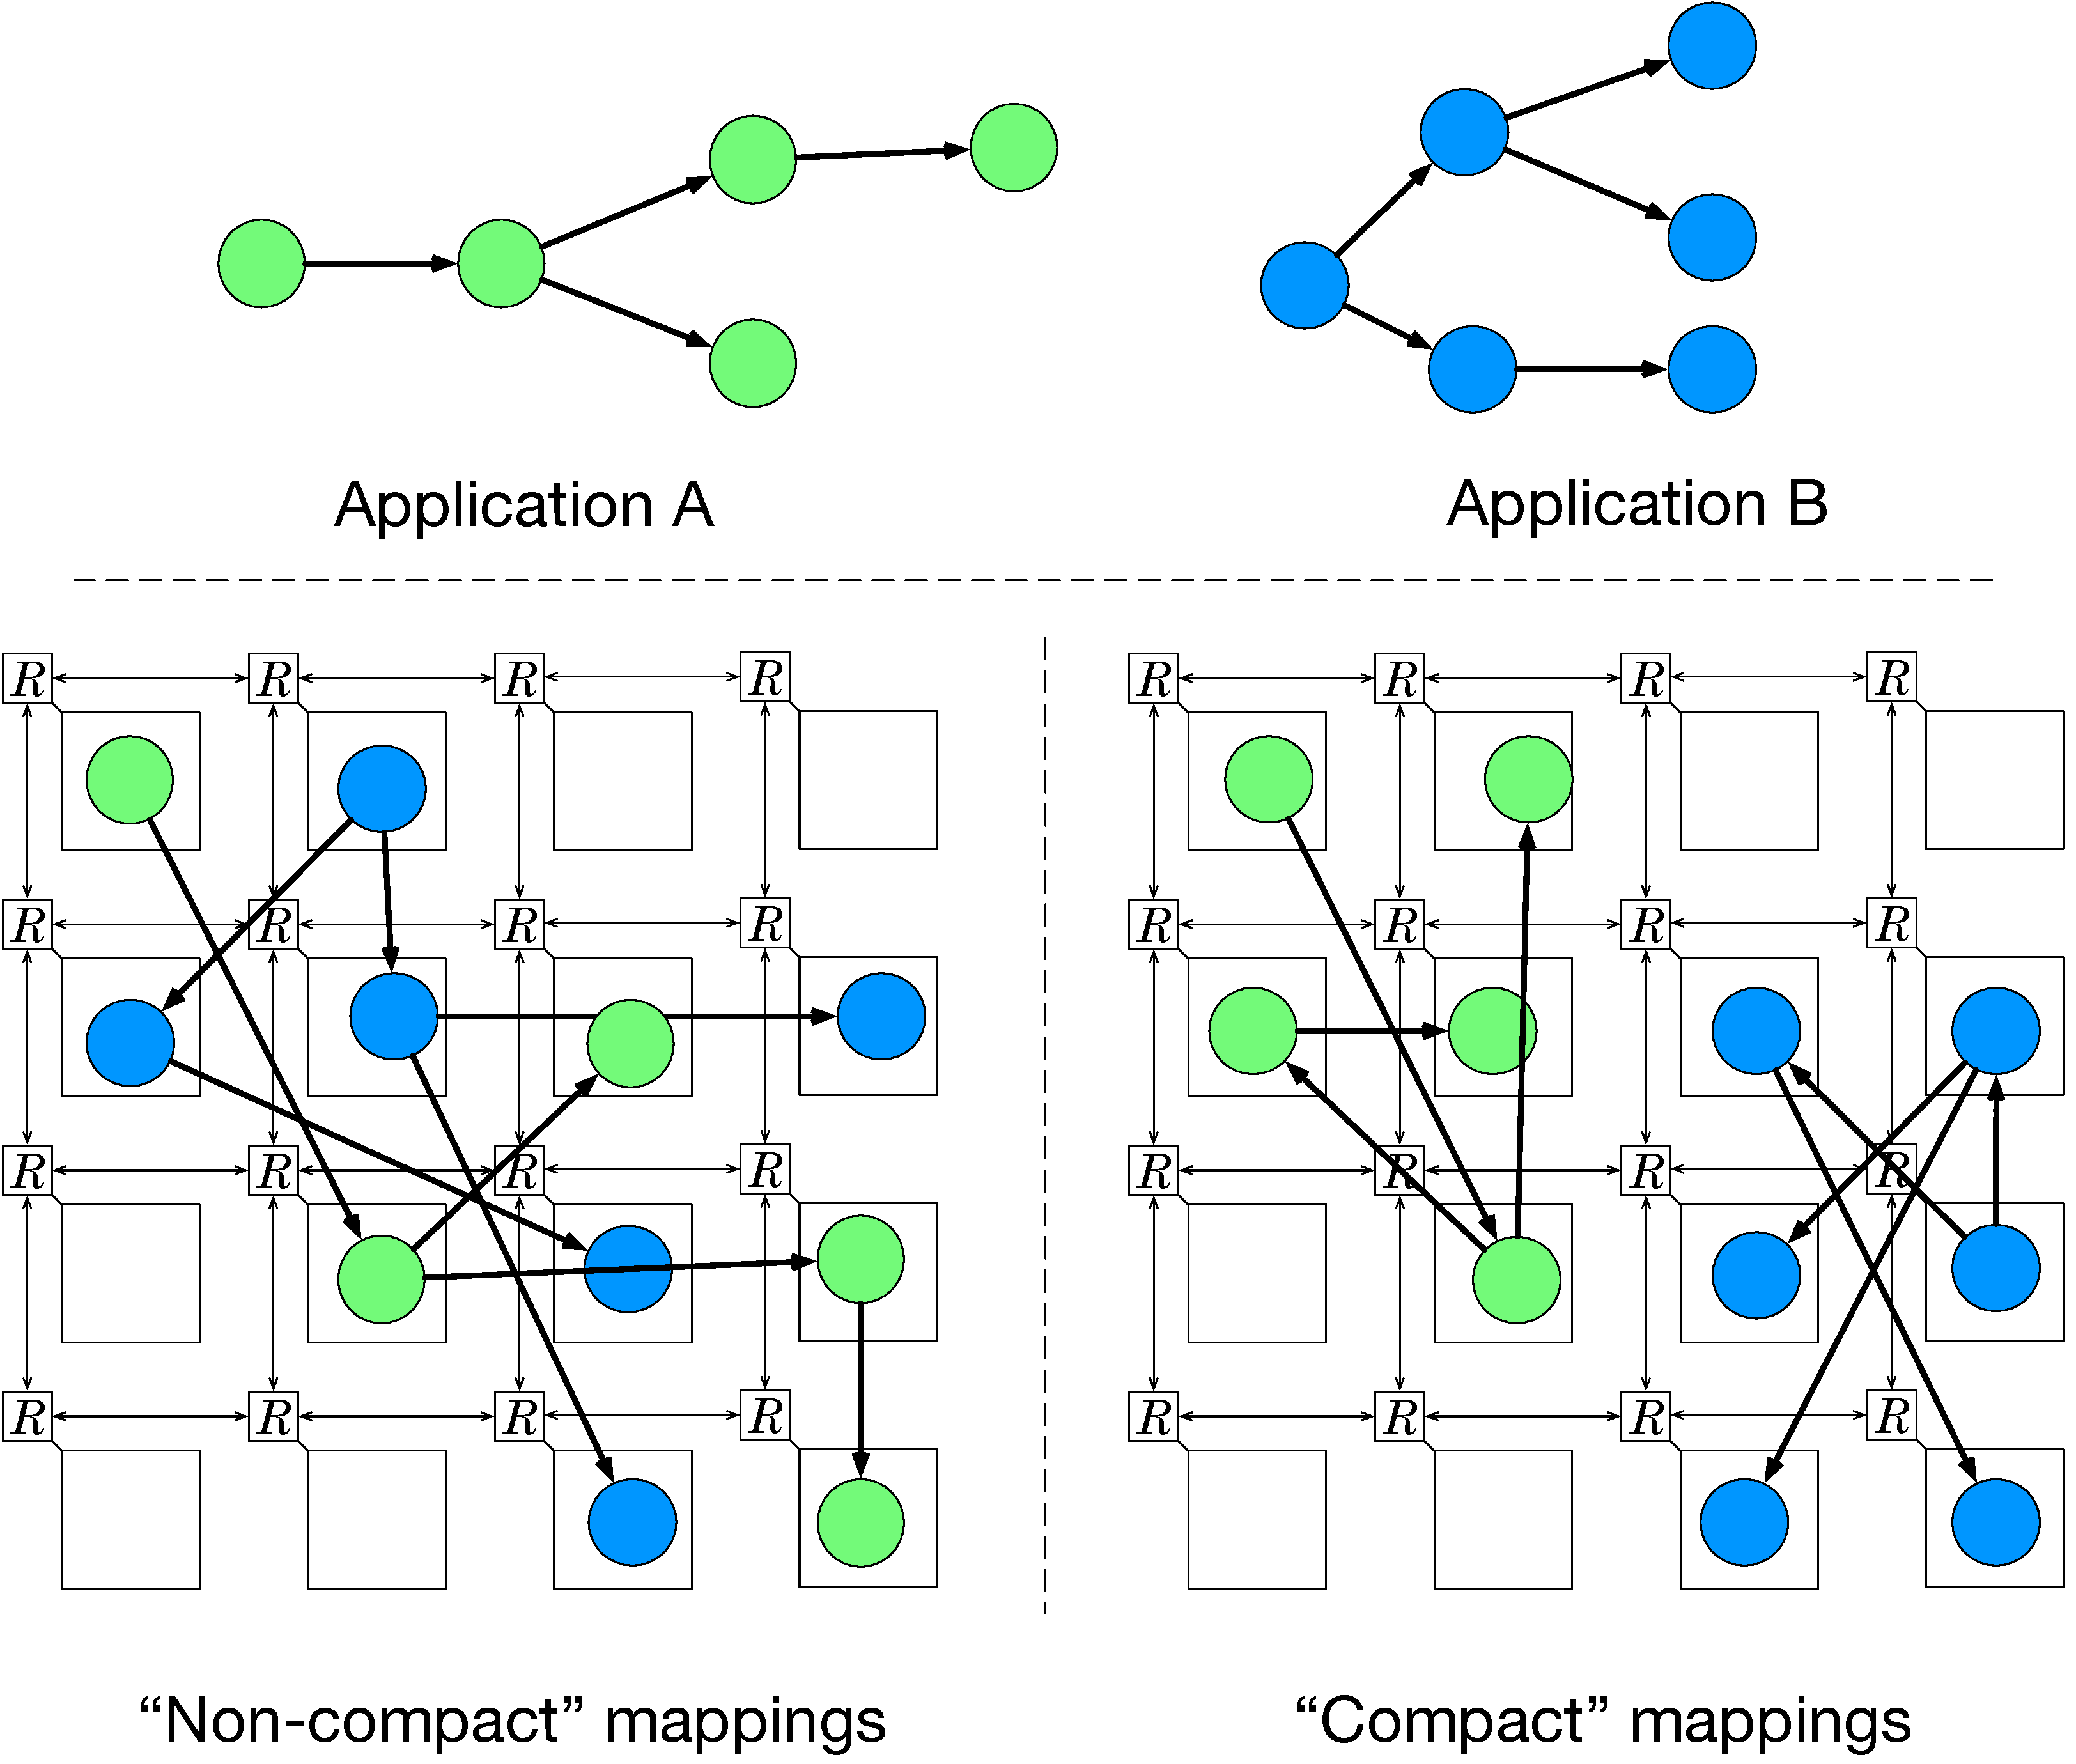
\includegraphics[width=0.6\textwidth]{figures/compact_intro.pdf}
	\caption{Equivalent mappings of two applications, one being compact and the other one not. Adapted from Figure~1 in~\cite{goens_samos19}.}
	\label{fig:compact_intro}
\end{figure*}

Figure~\ref{fig:compact_intro} illustrates the idea of compact mappings.
It depicts two variants for mapping the two application graphs depicted in the figure.
The particular property of these two variants is that they are equivalent from the point of view of the distances:
For any two connected nodes in any of the application graphs, the node distance in terms of number of hops between both nodes is identical in both mapping variants.
Intuitively, however, the mappings on the right are preferable to those on the left. 
Does this intuition translate to actual benefits in mappings?

To test this idea we used a SystemC-based \ac{NoC} simulator, Noxim~\cite{noxim}, which we modified to obtain more detailed statistics about the simulations~\cite{goens_samos19}.
In particular, we extracted the variance of the package delays in the simulation. 
We configured Noxim to simulate a $10 \times 10$ mesh topology with xy routing and worm-hole switching. 
This choice was made to mimic the routing of commercial platforms like the Tile-Gx series from Mellanox Technologies~\cite{technologies2015-tile-gx36-processor,technologies2015-tile-gx72-processor}, or Intel's Xeon Phi~\cite{tam2018-skylake-sp} or Scalable Platform~\cite{sodani2016-knights-landing}, or academic ones like OpenPiton~\cite{balkind2016-openpiton}.

If we execute the example from Figure~\ref{fig:compact_intro}, the non-compact example on the left actually outperforms the compact one on the right.
By closer inspection of the figure, this is because the distances within the application are very high.
In other words, the mappings depicted are simply bad mappings.
A lot of contention within the application offsets any gains from avoiding contention against other mappings.

However, while the motivational example is not very informative in terms of finding good mappings to combine, it does motivate the idea of compact mappings.
We used a heuristic to find such compact mappings in a regular mesh \ac{NoC}, while also ensuring they are not as bad as those in the example.
We do this by ensuring the communication costs are low within the application as well, using a greedy heuristic.

\begin{algorithm}
	\caption{A greedy heuristic for low-communication mapping in \ac{NoC}-based architectures. Adapted from Algorithm~1 in~\cite{goens_samos19}.}
	\label{algo:greedy_mapping}
	\begin{algorithmic}[1]
	  \Input{A connected application graph $K = (V_K,E_K)$, the size of the mesh $n$,
	  a set of occupied cores $X \subseteq \{1,\ldots,n\} \times \{1 \ldots, n \} =: V_A$}
	  \Output{ A mapping $m : V_K \rightarrow V_A$ }
	  \State CurNode $\leftarrow$ RandomFrom($V_A \setminus X$)
	  \State $v_0 \leftarrow \operatorname{Root}(K)$
	  \State mapping $\leftarrow~(v_0 \mapsto \text{CurNode})$
	  \State $X \leftarrow X \cup \{ \text{CurNode} \}$
	  \For{ $e = (n_1,n_2) \in \operatorname{BreadthFirstEdgeSearch}(K)$}
		  \State CurNode $\leftarrow$ mapping($n_1$)
		  \State $d \leftarrow \min_{d = 1 \ldots n} \{a \in V_A \setminus X \mid |a - \text{CurNode}| \leq d \} \neq \emptyset $
		  \State $q \leftarrow \operatorname{RandomFrom}(\{ a \in V_A \setminus X \mid |a - \text{CurNode}| \leq d  \})$
		  \State mapping$(n_2) \leftarrow q $
		  \State $X \leftarrow X \cup \{q\}$
	  \EndFor 
	  \Return mapping
	\end{algorithmic}
  \end{algorithm}


The heuristic is described in Algorithm~\ref{algo:greedy_mapping}.
We assume the application graph is (weakly) connected.
The heuristic then starts with any node in the application such that there is a path from it to every node in the application (\texttt{Root}).
It then randomly assigns an unused core to this node, subsequently iterating through the application graph in a breadth first fashion.
In this breadth-first search, it assigns cores such that the distance from a node to its predecessor is minimized in the mapping.
This greedy algorithm thus minimizes local communication, but it does not ensure that the communication is minimized globally for the whole application.

A central concept behind this algorithm is the set of cores marked as occupied, which can be initialized in a particular fashion to enforce the geometry of the mapping.
To produce compact mappings we mark every core as occupied, except for an $m \times m'$ rectangle such that $m,m' > |V|$, and we choose $\{m,m'\} \subseteq \{ \sqrt{|V|}, \sqrt{|V|}+1\}$ minimal with this property.
We compare these mappings to those produced without the additional rectangle constraint, which are low-communication mappings that are not necessarily compact.

To evaluate the concept of compact mappings we again used the Noxim simulation.
We generated random task graphs with a Gilbert random graph approach (cf. Section~\ref{sec:level_graphs}) with $10$ random applications with a variable number of tasks ($4$-$6$).
We simulated all $10$ applications running together in the system, multiple times, using different mapping strategies. 
For each application we then generated $100$ compact, $100$ non-compact (low-communication) and $100$ random mappings. 
We tested using a fixed packet size of $32$ flits (although the results were similar with packet sizes of up to $2^{12} = 4096$ flits).
Packages in Noxim were injected with a fixed injection rate (of packages per cycle), which we also varied between $10^{-2}$ and $10^{-5}$. 

\begin{figure}[h]
	\centering
   \resizebox{0.85\textwidth}{!}{\inputTikz{compact_latency.tex}}
	\caption{Comparison of latencies between compact, non-compact and random mappings. Adapted from Figure~2 in~\cite{goens_samos19}.}
	\label{fig:compact_latency}
\end{figure}

Figure~\ref{fig:compact_latency} shows the results of a comparison between compact, non-compact and random mappings. 
Each point reports the \emph{average network delays} over the course of the whole simulation for each of application and each mappings.\index{average network delay} 
We can see that for injection rates above $10^{-3}$ there is basically no difference between compact and non-compact mappings, and for the very high injection rate of $10^{-3}$ the difference is still negligible.

To make a better comparison, we designed an additional experiment that compared between two distinct scenarios.
In one scenario, the application was running alone in the system (isolated), and another one where it was executing alongside $9$ additional applications (joint).
In the case of the joint applications we report the values of one specific application (the same as in the isolated case), ignoring the rest.
The other applications only serve to create contention.

\begin{figure}[h]
	\centering
   \resizebox{0.85\textwidth}{!}{\inputTikz{compact_cases.tex}}
	\caption{Comparison between compact, non-compact and random mappings running isolation or with another 9 applications. Adapted from Figure~4 in~\cite{goens_samos19}.}
	\label{fig:compact_cases}
\end{figure}

Figure~\ref{fig:compact_cases} shows the results of this experiment comapring applications running in isolation and with contention.
For an injection rate of $10^{-5}$ contention is so low that it makes no difference between two cases (except for random mappings).
When increasing the rate to $10^{-4}$, while contention does affect applications, the compactness of the mappings still makes no difference.
Compact mappings do perform slightly better only for very high injection rates ($10^{-3}$) and significantly better for extremely high injection rates $10^{-2}$.
Note that an injection rate of $10^{-2}$ every task is sending a package in average every $100$ cycles, which is arguably of no practical relevance. 

\begin{figure*}[th]
	\centering
	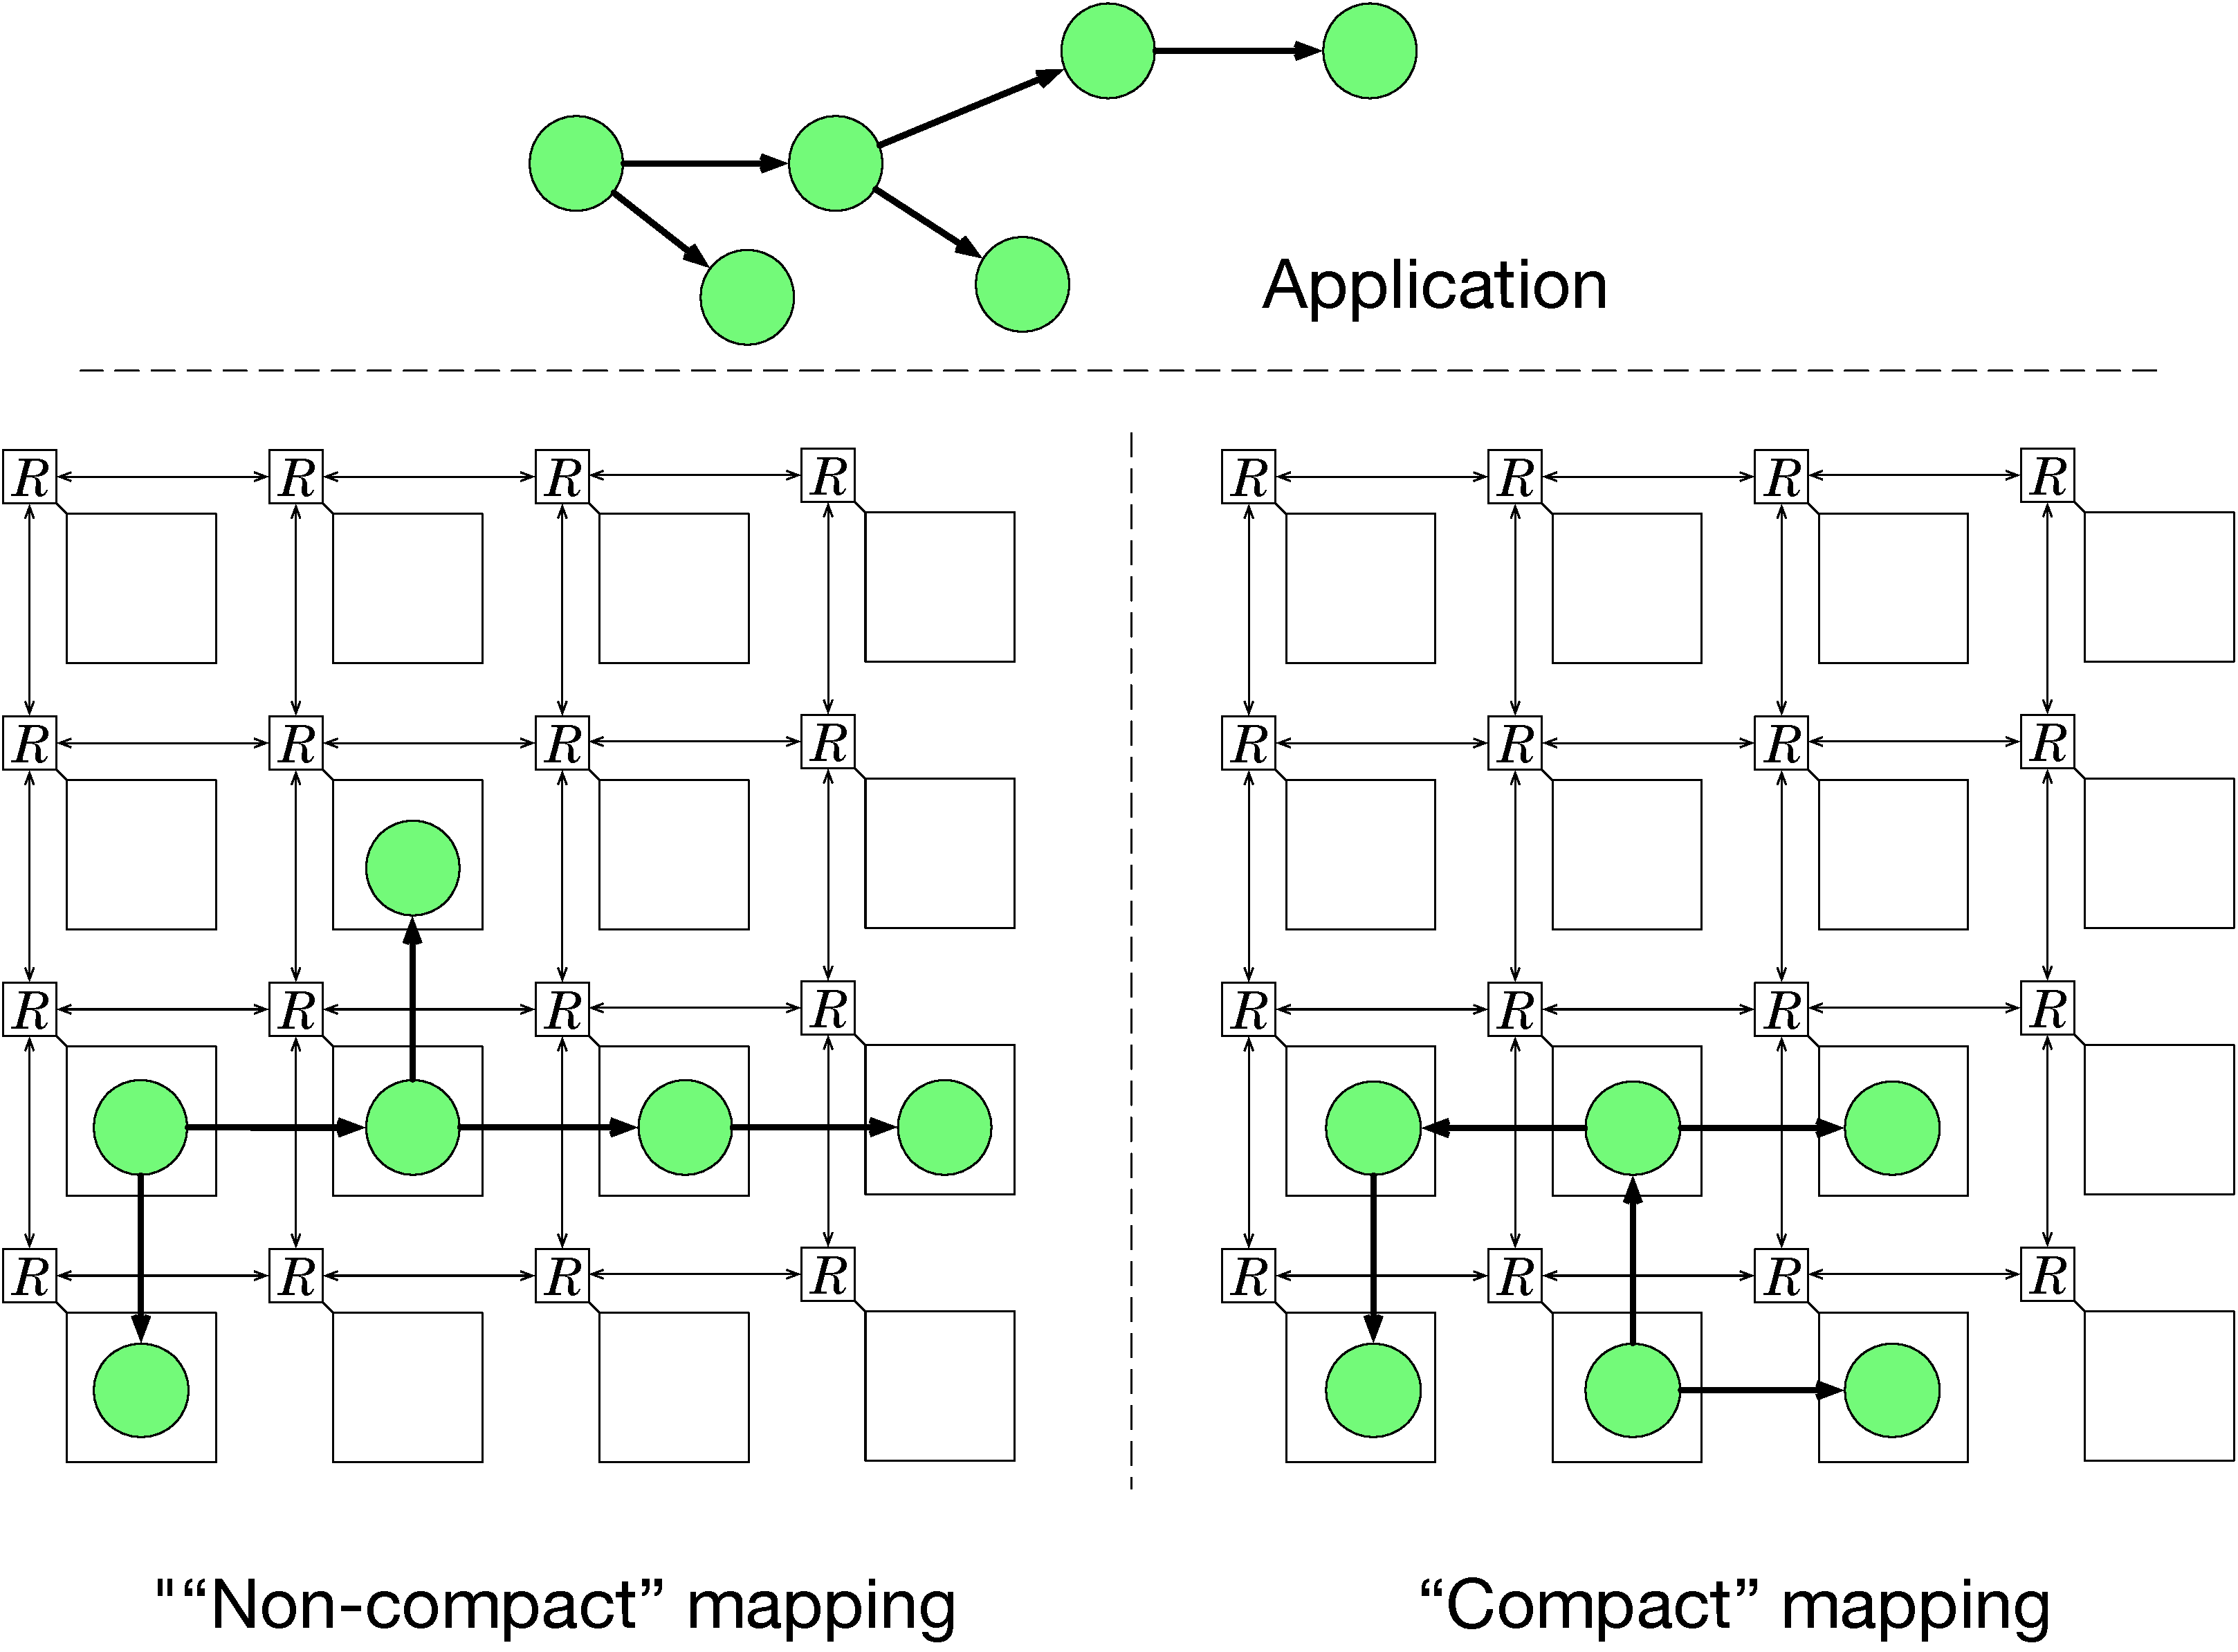
\includegraphics[width=0.6\textwidth]{figures/topology_vs_geometry.pdf}
	\caption{Two equivalent mappings that yield good performance. Adapted from Figure~5 in~\cite{goens_samos19}.}
	\label{fig:topology_vs_geometry}
\end{figure*}

From these experiments we can conclude that compact mappings are not particularly useful. 
The improvements they bring in reducing contention are not relevant in practice, since the amount of contention required for the compactness to make a difference is unrealistically high.
Figure~\ref{fig:topology_vs_geometry} shows a comparison between a typical example of two low-communication mappings, a compact one and a non-compact one. 
These are the kinds of mappings that result from Algorithm~\ref{algo:greedy_mapping} (with and without the additional compactness constraint).
These two mappings are good in the sense that they produce low average network delays, as they minimize the distance that the tokens travel and the contention they generate.
While their geometries are very different, one being compact and the other one not, their topologies are identical. These two mappings are also equvialent in the same sense as the mappings in Figure~\ref{fig:compact_intro} were.
The number of hops between any two nodes is identical for both.
A key takeaway thus is that the topology of the mapping is much more important than its geometry, as seen by comparing the compact mapping in Figure~\ref{fig:compact_intro} with the non-compact one in Figure~\ref{fig:topology_vs_geometry} (note that the application is sligthly different).